\subsection{Figures with two images}

\begin{figure}[ht!]
    \centering
    \begin{subfigure}
        \centering
        \raisebox{-0.5\height}{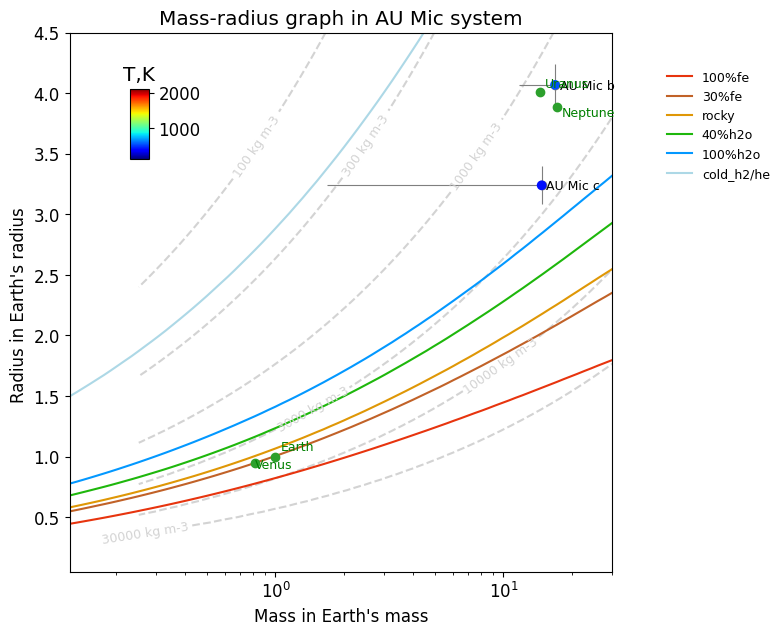
\includegraphics[width=0.45\textwidth]{./img/AU Mic.png}}
    \end{subfigure}
    \hfill
    \begin{subfigure}
        \centering
        \raisebox{-0.5\height}{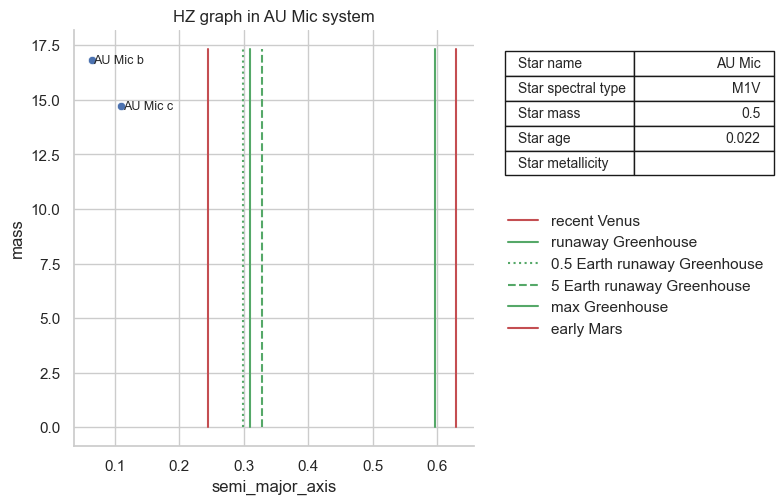
\includegraphics[width=0.45\textwidth]{./img/AU Mic_with_HZ_edges.png}}
    \end{subfigure}
    \caption{AU Mic charts}
    \label{charts-au-mic}
\end{figure}

\begin{figure}[ht!]
    \centering
    \begin{subfigure}
        \centering
        \raisebox{-0.5\height}{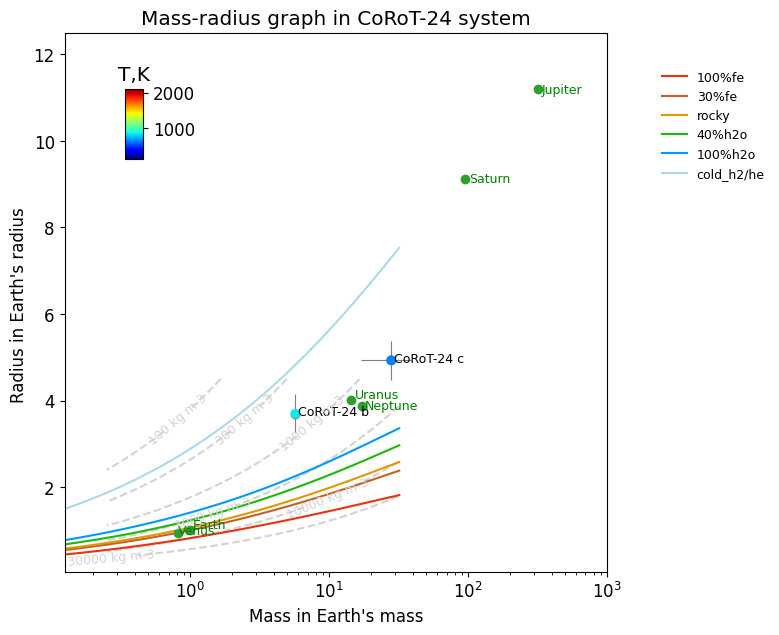
\includegraphics[width=0.45\textwidth]{./img/CoRoT-24.png}}
    \end{subfigure}
    \hfill
    \begin{subfigure}
        \centering
        \raisebox{-0.5\height}{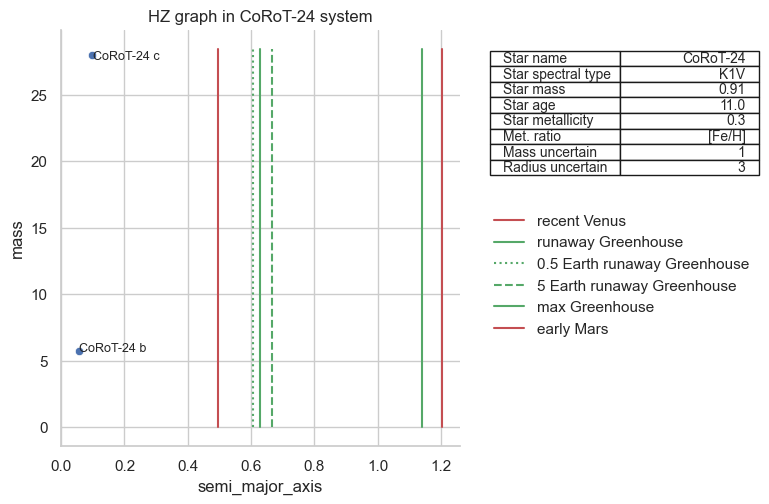
\includegraphics[width=0.45\textwidth]{./img/CoRoT-24_with_HZ_edges.png}}
    \end{subfigure}
    \caption{CoRoT-24 charts}
    \label{charts-corot-24}
\end{figure}
